\documentclass[12pt,oneside]{article}
\usepackage[spanish,es-nodecimaldot]{babel}
\usepackage[utf8]{inputenc}
\usepackage[spanish]{babel}
\usepackage[T1]{fontenc}
\usepackage{lmodern}
\usepackage{xurl} 
\usepackage{geometry}
\usepackage{setspace}
\usepackage{hyperref}
\usepackage{graphicx}
\usepackage{csquotes}
\usepackage{microtype}
\geometry{letterpaper, margin=2.5cm}
\hypersetup{
    colorlinks=true,
    linkcolor=black,
    citecolor=black,
    urlcolor=black
}

\begin{document}
\begin{figure}[t]
    \centering
    
\includegraphics[width=0.2\textwidth]{imagenes/utal.png}
\end{figure}

\begin{titlepage}
    \centering
    \Large \textbf{UNIVERSIDAD DE TALCA} \\[4pt]
    \large FACULTAD DE INGENIERÍA \\
    \large ESCUELA DE INGENIERÍA CIVIL EN COMPUTACIÓN \\[2cm]
    \LARGE \textbf{Aplicación web para el apoyo del proceso de fabricación de muebles a medida} \\[1cm]
    \large ANGEL NICOLÁS BRAVO MUÑOZ\\[4cm]
    \begin{flushleft}
    \large Profesor Guía: FRANCISCO ARIAS \\[2cm]
    
    \large Formulación de proyecto de titulación. \\[1.5cm]
    \large Curico –
Chile \\[6pt]
    \large SEPTIEMBRE 2025
    \end{flushleft}
\end{titlepage}

\pagenumbering{roman}
\tableofcontents
\listoffigures
\clearpage
\pagenumbering{arabic}

\section{Resumen}
\onehalfspacing
\begingroup
\noindent En zonas rurales, el diseño y fabricación de muebles suele depender de métodos tradicionales que dificultan la estimación precisa de costos y el aprovechamiento eficiente de materiales. La falta de herramientas digitales accesibles limita la capacidad de los artesanos y pequeños fabricantes para planificar, optimizar y competir en mercados más exigentes.\\

\noindent En zonas rurales, el diseño y fabricación de muebles suele depender de métodos tradicionales que dificultan la estimación precisa de costos. La falta de herramientas digitales accesibles limita la capacidad de los artesanos y pequeños fabricantes para planificar, optimizar y competir en mercados más exigentes.\\

\noindent Desarrollar una plataforma web que permita diseñar muebles en 2D, estimar costos automáticamente y optimizar el uso de materiales, todo desde una interfaz sencilla y accesible. La solución está orientada a mejorar la productividad de usuarios en contextos rurales, facilitando la transición hacia procesos más eficientes y digitalizados.

\endgroup

\subsection{Diseño de la propuesta}
\subsubsection{Contexto}
\onehalfspacing
\begingroup
El rubro de mueblería abarca la industria dedicada al diseño, fabricación, comercialización y distribución de muebles para diversos espacios como hogares, oficinas y más. Los muebles pueden estar hechos de madera, metal, plástico, vidrio, cuero, telas o combinaciones de estos [21].\\

\noindent Además se encuentran 2 tipos de muebles:
\begin{itemize}
    \item \textbf{Fabricación estándar en serie}: Los cuales se basan en la producción masiva con medidas y diseños estandarizados, como por ejemplo IKEA[21].

    \item  \textbf{Fabricación de mueble a medida o artesanal}: Se enfoca en crear diseños únicos adaptados a las necesidades especifícas del cliente.[1]
\end{itemize}

\noindent Según el estudio de Rodrigo Vidal 2017[1] sobre la fabricación y comercialización de muebles multifuncionales en Chile, más del 95\% de los encuestados manifestó la necesidad de optimizar el espacio en sus viviendas, lo que representa una oportunidad para el rubro de fabricación de muebles a medida en comparación con los muebles pre-fabricados de medidas estándar. Adicionalmente, un 55,43\% considera que el mobiliario actual no cumple con estas necesidades. Además, los atributos más valorados por los consumidores son el estilo y diseño, la multifuncionalidad y la exclusividad.\\

\noindent En un estudio se evidencia que el sector mueblero en Chile es parte de las actividades económicas de relevancia creciente, dado que es una demanda en aumento por la clase media para amueblar su casa con su decoración y estilo deseado, con un mercado estimado en USD 660 millones en 2023 y una proyección de crecimiento anual de 4,8\% entre 2025 y 2034, y así alcanzar un valor de 1,006.82 millones de USD en 2034.[2] \\

\noindent A nivel regional, los parámetros son diferentes, ya que en la Región Metropolitana las ventas de muebles registraron una caída acumulada de 2,6 \% en los primeros meses de 2025 [3] mientras que en regiones como Valparaíso y La Araucanía se observó un crecimiento positivo del 5,9 \% durante el mismo período [4].\\

\noindent Para el desarrollo de este proyecto nos centraremos en el desarrollo de muebles a medida lo cual se detallará en los siguientes parrafos.\\

\noindent La naturaleza de este oficio nace al traspasar las técnicas de diseñar y crear muebles de generación en generación, al no ser un tipo de enseñanza formal, cada mueblista tiene que buscar su manera de poder diseñar o plantear sus ideas, por lo  que están lo que usan papel, al ser una herramienta tangible, generando un lento proceso de los cálculos y dimensiones para hacer una entrega de un presupuesto de material.\\

\noindent La manera más común de actuar en este rubro es que contacten al mueblista, entre ambas partes acuerden una hora en común para la visita de medición en donde el cliente le proponga lo que necesita y requiere para que el mueblista en base a eso plantee su diseño de un mueble que cumpla con sus requerimientos, lo que muchas veces suele ser un boceto rápido para que el cliente tenga una idea del producto que obtendrá. Una vez planteada la idea con las medidas, el mueblista procede a realizar el diseño más técnico para calcular la cantidad de material que va a usar con sus correspondientes medidas, por lo que dependiendo de las dimensiones y complejidad del mueble, pudiendo demorar desde 2 horas hasta 8 horas, en ese momento se hace la cotización al proveedor para recién contactar al cliente y decirle que se va a necesitar una cantidad de dinero para material. A continuación, el cliente escoge si desea el mueble o no, en el caso de que lo acepte se va con el distribuidor a comprar la plancha en este caso dimensionada por el mismo distribuidor, esto puede demorar de 1 a 3 días hábiles. Una vez recibido el material se comienza el armado del mueble el cual puede demorarse desde un par de días hasta semanas, dependiendo de las piezas y la complejidad del mismo. Para cuando esté listo se coordina con el cliente para ir a dejar el mueble en la casa y lugar solicitado por el cliente. La Figura 1 describe el proceso de fabricación de muebles a medida anteriormente explicado.\\

\begin{figure}[htbp]
    \centering
    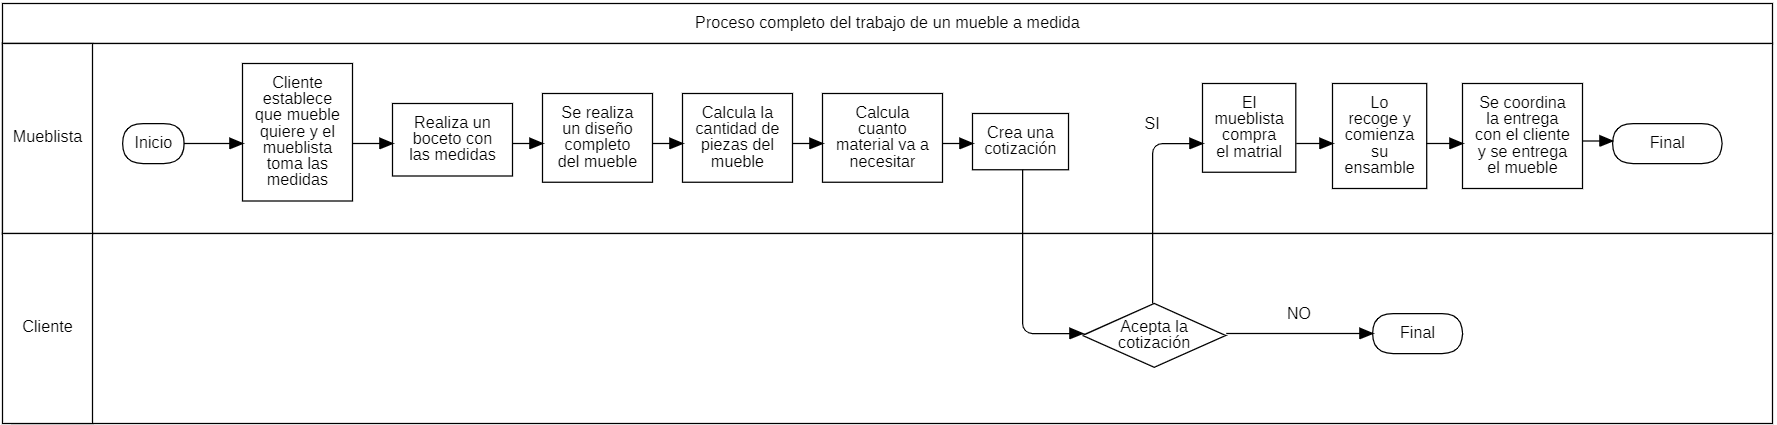
\includegraphics[width=1\textwidth]{imagenes/Diagrama formulación.png}
    \caption{Diagrama del proceso de solicitud y construción de mueble a medida.}
    \label{fig: diagrama}
\end{figure}

\noindent Esta información respalda la pertinencia de desarrollar una plataforma digital que permita al mueblista diseñar muebles a medida en un entorno 2D, visualizando en tiempo real el impacto estético y funcional de sus decisiones, y recibiendo una cotización ajustada a materiales, dimensiones y acabados seleccionados. La integración de diseño y presupuesto responde directamente a las brechas detectadas en el mercado, la optimización del espacio siguen siendo necesidades insatisfechas.\\

\subsubsection{Problema}
\begingroup
\small
El proceso de fabricación de muebles a medida es generalmente trasmitido de generación en generación. La oportunidad de mejora o modernización es lenta o muy básica, ya que hay mueblistas que trabajan con bocetos en papel, requieren de mucha precisión en las escalas al momento del dibujo, lo que, en muchos casos se ve afectado por las limitaciones educativas presentes en zonas rurales [1]. Si se considera un mueblista que sepa hacer los diseños, el tiempo que invierte al ser todo manual es prolongado ya que se tiene que hacer el diseño para posteriormente estimar cantidad de cortes (segmentos del material a utilizar) son requeridos según el tamaño de la “plancha” (tamaño original o máximo del material en cuestión), por lo cual para lograr un presupuesto completo al detalle es un proceso que requiere dedicarle mucho tiempo y ser muy milimétrico.\\

\noindent Por esto es que hay mueblistas que fueron criados a partir de este rubro/oficio. A pesar de existir herramientas que puedan facilitar su trabajo, van a preferir no pagar por una aplicación que no saben si van a entender o que no le puedan sacar el suficiente provecho [19]. Se deja de lado a los mueblistas independientes, además en general por la tardanza de los procesos de cotizaciones iniciales muchas veces no se puede competir con las grandes tiendas, que al tener un stock o que solo requieran de la entrega, genera mucha diferencia comparativamente en los tiempos de respuesta [20].

\subsubsection{Propuesta de solución}
\begingroup
La solución propuesta consiste en el diseño y desarrollo de una plataforma web para el diseño 2D de muebles y cálculo de material, orientada a apoyar y optimizar el tiempo en el rubro del mueblista o carpintero artesanal. Este sistema deberá contar con un espacio de diseño de muebles el cual disponga de los elementos comunes del proceso de fabricación de muebles a medida, por ejemplo espacios modulares de cajoneras, espacios de repisas, colgadores, cubiertas, etc., en donde el mueblista pueda escoger cada módulo que necesite, simplificando su usabilidad solo teniendo que modificar las dimensiones (alto, ancho y profundidad) del mueble de acuerdo con los requerimientos del usuario, sin necesidad de ensamblar cada pieza de forma individual. Una vez definido el diseño, el sistema deberá calcular automáticamente los materiales necesarios para su fabricación (por ejemplo, el número de planchas de melamina requeridas) y generar un listado detallado de materiales.\\

A continuación se describen las etapas involucradas en la elaboración de una cotización para la fabricación de un mueble, junto con sus tiempos estimados y propuestas de optimización:

\begin{itemize}
    \item \textbf{Etapa de diseño:} El mueblista realiza un boceto con las medidas de alto, ancho y profundidad del mueble solicitado. Este proceso puede tardar entre 2 a 4 horas, dependiendo de la complejidad del diseño y la cantidad de piezas involucradas. Se propone optimizar esta etapa mediante el uso de la aplicación web, permitiendo realizar el diseño de forma más ágil y digital. Se espera una reducción del tiempo de diseño de un 25\%, logrando tiempos entre 1 hora y 45 minutos a 3 horas.

    \item \textbf{Etapa de cubicación:} A partir del diseño, se calcula la cantidad de cortes necesarios y el volumen de material requerido. Este proceso actualmente se realiza de forma manual y puede tardar entre 2 a 8 horas, dependiendo de la cantidad de piezas y cortes. Con la aplicación web, se busca que la cubicación se realice automáticamente al finalizar el diseño, reduciendo este tiempo a solo minutos, lo que representa una mejora de aproximadamente 90\%.

    \item \textbf{Tiempo total de cotización:} Sumando ambas etapas, el tiempo promedio para entregar una cotización es de aproximadamente 9 horas (3 horas en diseño + 6 horas en cubicación). Con la implementación de la solución propuesta, este tiempo se reduciría significativamente, permitiendo entregar cotizaciones en menos de 4 horas.

    \item \textbf{Impacto en el proceso completo:} Considerando que la fabricación de un mueble puede tardar entre 2 a 10 días, la optimización de las etapas de diseño y cubicación permitiría una mejora global del proceso de en un 15\%.
\end{itemize}

Además se busca contar con una base de datos del historial de muebles para que el mueblista al momento del diseño pueda escoger un mueble ya hecho y modificar las medidas del mueble en general o modificar los módulos según corresponda.\\

Una vez hecho el cálculo de material se puedan modificar los detalles de la cotización para que el cliente vea el cambio del valor total dependiendo del color, grosor o composición del material.

A su vez la aplicación tendrá con un módulo de estadística básica que permitirá registrar y visualizar los periodos del año con mayor demanda de muebles. Este módulo ofrecerá indicadores como el máximo, promedio y mínimo de ventas, segmentados por mes o por año.


\subsection{Objetivos}
\begingroup
\subsubsection{Objetivo General}

Optimizar el proceso de diseño y cubicación en la fabricación de muebles a medida, mediante el desarrollo de una aplicación web intuitiva que sirva como herramienta para la creación de planos personalizados, el cálculo de materiales y la generación de cotizaciones precisas.\\

\subsubsection{Objetivos específicos}
\begin{itemize}
\item Implementar una aplicación web que provea de un espacio de diseño en dos dimensiones (2D) orientado a muebles para que el fabricante pueda generar diseños personalizados a la necesidad del cliente.

\item Implementar el módulo de cubicación que apoye al fabricante en el cálculo de materiales y costos, agilizando el proceso de propuesta para el cliente. 

\item Desarrollar un respositorio de muebles que permita guardar, reutilizar y modificar diseños previamente realizados.

\item Implementar una biblioteca de materiales, colores, grosores y accesorios que permita y facilite la personalización de los diseños.

\item Automatizar la generación y envío de cotizaciones detalladas e interactivas para que el cliente o mueblista elija entre un abanico de posibilidades.

\item Reducir el tiempo en el proceso de fabricación de muebles a medida en un 15\% respecto al método manual.  

\item Implementar un módulo de estadísticas simples.
\end{itemize}
\endgroup

\subsection{Alcances}
\begingroup
\small
\begin{itemize}
\item La plataforma podrá ser utilizada en entorno web responsive.

\item La aplicación no será nativa móvil.

\item Para la toma de requerimientos se contactará con un mueblista artesanal de la localidad de Teno.

\item La plataforma no generará modelos 3D de los muebles diseñados.

\item La aplicación contará con un área de diseño 2D especializada para muebles modulares.

\item La plataforma no realizará envíos físicos de materiales ni coordinará logística de entrega.

\item La aplicaión no incluirá gestión de clientes.

\item Requerirá que los usuarios tengan conexión a Internet para acceder a la plataforma.

\item La plataforma no procesará pagos ni gestionará transacciones financieras.

\end{itemize}
\endgroup



\subsection{Plan de Trabajo}
\begingroup
\small
 A continuación se presenta el plan de trabajo del proyecto.
\subsubsection{Descripción de etapas del proyecto}

En esta sección se presentan las etapas de el proyecto, tareas más imporantes y la cantidad de semanas de duración que implicará realizar cada etapa.
\begin{enumerate}
\item Requerimientos (1 semana)
    \begin{itemize}
        \item Capturar requerimientos mediante entrevista.
    \end{itemize}

\item Planificación (2 semanas)
\begin{itemize}
    \item Creación y estimación de historias de usuario.
    \item Definición de tecnologías.
    \item Diseño de modelo de base de datos, mockups y arquitecturas.
\end{itemize}
    
\item Implementación (19 semanas)
\begin{itemize}
    \item Configuración inicial de proyecto.
    \item Implementar módulo de diseño de muebles.
    \item Implementar módulo de visualización de cortes.
    \item Implementar módulo de gestión de cotización.
    \item Implementar módulo de muebles realizados.
    \item Implementar módulo de biblioteca de materiales.
    \item Integración de los módulos desarrollados.
   \item  Implementar módulo estadística.
\end{itemize}

    
\item Evaluación (2 semanas):
\begin{itemize}
    \item Aplicar pruebas de caja negra.
    \item Correcciones de aplicación.
    \item Aplicar prueba de usabilidad con su encuesta.
\end{itemize}

 \item Conclusión (2 semanas):
 \begin{itemize}
    \item Comparar métricas de entrevista inicial y final.
    \item Realizar conclusiones y completar documento.
 \end{itemize}

\end{enumerate}
Quedando así un total de 26 semanas para el desarrollo del proyecto entre los 2 semestres dejando una semana para una revisión exhaustiva del documento. Para mayor detalle de la planificación revisar la Carta Gantt.

\subsubsection{Tareas para objetivos específicos}
Para cumplir los objetivos específicos se tiene en cuenta las siguientes
 acciones para cada uno de ellos:

\begin{itemize}
\item Implementar una aplicacion web que tenga un espacio de diseño 2D orientado a muebles para que el mueblista pueda plantear los diseños personalizados a la necesidad del cliente.
\begin{enumerate}
\item Etapa 3: Implementar módulo de diseño de muebles.
\item  Etapa 3: Implementar módulo de gestión de cotización.
\end{enumerate}

\item Implementar el apartado de cubicación que apoye el cálculo de materiales y costos, agilizando el proceso de propuesta para el cliente.
\begin{enumerate}
\item Etapa 3: Implementar módulo de visualización de cortes.
\end{enumerate}

\item Desarrollar un historial de muebles que permita guardar, reutilizar y modificar diseños previamente realizados.
\begin{enumerate}
\item Etapa 3: Implementar módulo de muebles realizados.
\end{enumerate}

\item Implementar una biblioteca de materiales, colores, grosores y accesorios que permita y facilite la personalización de los diseños.
\begin{enumerate}
\item Etapa 3: Implementar módulo de biblioteca de materiales.
\end{enumerate}

\item Generar cotizaciones detalladas e interactivas para que el cliente o mueblista elija entre un abanico de posibilidades.
\begin{enumerate}
\item Etapa 3: Implementar módulo gestión de cotizaciones.
\end{enumerate}

\item Optimizar el tiempo en el proceso de fabricación de muebles a medida en un 15\% respecto al método manual.  
\begin{enumerate}
\item Etapa 3: Implementar módulo de diseño de muebles.
\item Etapa 3: Implementar módulo de visualización de cortes.
\item Etapa 3: Implementar módulo de gestión de cotización.
\item Etapa 3: Implementar módulo de muebles realizados.
\item Etapa 3: Implementar módulo de biblioteca de materiales.
\end{enumerate}

\item Implementar un módulo de estadísticas simples.
\begin{enumerate}
\item Etapa 3: Implementar módulo estadística.
\end{enumerate}
\end{itemize}

\section{Marco Teórico}
Este capitúlo está orientado a describir conceptos necesarios para entender el foco del proyecto. Además, se explicarán las tecnologías que serán parte del proyecto.

\subsection{Conceptos}
\begin{itemize}
    \item Cubicación: es un término fundamental en arquitectura, ingeniería y construcción. Es el proceso técnico de medir y calcular las cantidades de materiales, mano de obra y elementos que se necesitarán para ejecutar un proyecto u obra.\\
    Teniendo como objetivo principal cuantificar el proyecto para para elaborar un presupuesto preciso, planificar la compra de materiales y programar los trabajos.
\end{itemize}

\subsection{Tecnologías}
\begin{itemize}
    \item React: React es un framework de mantenido por Meta y la comunidad, utilizada para construir interfaces de usuario (UI) interactivas y reutilizables. Su enfoque se basa en el concepto de "componentes", que son partes o piezas de código encapsuladas e independientes que manejan su propio estado.\\
    Por este motivo, React ha sido seleccionado como el framework ideal para la implementación de la solución propuesta.
    
    \item MongoDB: Es un sistema gestor de bases de datos No SQL, orientado a documentos. A diferencia de las bases de datos relacionales o SQL que usan tablas, filas y relaciones, MongoDB almacena los datos en documentos flexibles similares a JSON (llamados BSON), lo que permite manejar datos completos y semiestructurados de forma natural.\\
    Es por esta flexibilidad en el esquema que permite guardar, reutilizar y modificar diseños más eficiente y escalable que intentar normalizar esa información en múltiples tablas relacionales.
    
    \item Konva.js: Es una librería de Javascript que extiende las capacidades del "Canvas" 2D de HTML. Permitiendo crear gráficos 2D interactivos y de alto rendimiento, trabajando con las formas (rectángulos, círculos, etc.) como "objetos" en un "escenario" (Stage) y "capas" (Layers). Facilitando la gestión de eventos (arrastrar, soltar), animaciones y transformaciones de objetos.\\
    Es por estos motivos que Konva.js es de las mejores opciones para usar en comparación de Fabric.js que fue otra opción a utilizar, pero por rendimiento, usabilidad y compatibilidad con React es que es la mejor opción a utilizar.

    \item Git: Es un sistema de control de versiones distribuido, gratuito y de código abierto, diseñado para manejar todo, desde proyectos pequeños hasta proyectos muy grandes, con velocidad y eficiencia.
    Se usara para llevar el control de las actualizaciones del proyecto y 

 \end{itemize}
\subsection{Estado del arte}
En cuanto al estado del arte del proyecto, existen distintos tipos de herramintas tanto de paga como gratuitas, a continuación, se mencionan y decriben algunas herramientas reconocidas que estan relacionadas con el proyecto.

\noindent 1. \textbf{AutoCAD} [5].  Es un software de diseño de paga que se utiliza para dibujar, diseñar y modelar en 2D y 3D de forma precisa con sólidos, superficies, objetos de malla, características de documentación, etc. Incluye características para automatizar tareas y aumentar la productividad, como la comparación de dibujos, el recuento, la adición de objetos y la creación de tablas.\\

\noindent 2. \textbf{IKEA PLanner} [6]. Es un software web de IKEA que se encarga de dar ideas según el catálogo de IKEA, en donde se tiene un plano 3D de un espacio genérico de cocina, baño, etc. el cual permite agregar muebles de IKEA para ajustarlo según las necesidades del cliente. \\

\noindent 3. \textbf{Cabinet Vision} [7]. Es un software de HEXAGON el cual se utiliza para el diseño de muebles 2D y 3D incluyendo el 'listado de cortes', automatizando la exportación a diferentes formatos para las solicitudes de material. Esta aplicación solo es de uso empresarial.\\

\noindent 4. \textbf{Moblo} [8]. Es un software que se utiliza para crear diseños 3D de un mueble según las necesidades a partir de figuras simples, permitiendo modificar su color o tipo de material, de uso gratuito. \\

\noindent 5. \textbf{Cut list} [9]. Es un software que se utiliza para cubicar la lista de cortes de los muebles en la plancha de manera visual y así saber cuanto material se va a usar en el ensamble del mueble. Se ingresan todos los valores de manera manual y también lo que se pierde por corte. Además permite exportar lo listado en PDF o PNG.\\ 

\noindent 6. \textbf{SketchUp} [10]. Es un software que se utiliza para modelado 2D y 3D de estructuras, ya sea cons\-trucción, muebles o diseño de interiores, siendo de paga para profesionales, con posibilidad de vista en realidad virtual (VR).\\

\noindent 7. \textbf{Opticutter} [11]. Es un software web que se usa de calculadora de hoja de corte en línea la cual obtiene una solución utilizando el algoritmo de optimización adecuado. 
\endgroup


\section{Metodologías}
En este capítulo se presentan las metodologías de desarrollo y de evaluación para
el proyecto
\begingroup
\subsection{Metodologías de desarrollo}
Dado que este proyecto será desarrollado de manera individual, se realiza una comparación entre diferentes metodologías ágiles destacando tres opciones: Kanban[10], Personal Extreme Programming (PXP)[11] y Lean Startup[12], todas son independientes del lenguaje de programación o framework seleccionado. Estas metodologías comparten el enfoque ágil.\\

\noindent \textbf{Personal Extreme Programming (PXP)}: Adaptación individual de la metodología Extreme Programming (XP). PXP usa prácticas como desarrollo incremental, pruebas automatizadas, diseño simple y refactorización continua, pero ajustadas a un entorno unipersonal.\\

\noindent Para este proyecto se elige Personal Extreme Programming (PXP) dado que se adapta a las características requeridas en el contexto. Además PXP se centra en la calidad del código desde el inicio, además de que permite avanzar en ciclos cortos, lo que facilita ajustes constantes y mejora continua proporcionando flexibilidad durante el desarrollo.\\

\noindent Para el desarrollo de esta propuesta se seguirán distintas fases que contempla la metodología:\\

\noindent \textbf{Requerimientos}: Durante esta etapa se captan los requisitos del proyecto en conjunto con el cliente.\\

\noindent \textbf{Planificación}: Durante esta fase se desarrolla la creación y estimación de las historias de usuarios, la elección de tecnologías a utilizar, diseño de mockups y arquitectura.\\

\noindent \textbf{Iteración}: Durante esta etapa se indica la inicialización de cada iteración o ciclo, la cual puede durar entre 1 y 4 semanas.\\

\noindent \textbf{Diseño}: Durante esta fase se desarrolla el diseño lógico de módulos y funciones correspondientes a cada iteración.\\ 

\noindent \textbf{Implementación}: Durante esta fase se realiza el desarrollo mediante programación de las historias de usuario asociadas a una tarea, para salir de esta fase debe funcionar sin errores y pasar todas las pruebas unitarias, en caso de no ser así se debe refactorizar el código realizado.\\

\noindent \textbf{Sistema de Pruebas}: Durante esta fase se realiza el testeo para validar las funcionalidades desarrolladas durante la iteración y se debe verificar si la solución implementada con los requisitos iniciales del proyecto.\\

\noindent \textbf{Retrospectiva}: Esta fase demarca el final de cada iteración, se realiza un análisis de los datos recopilados durante las fases y de las propuestas de mejora. Esta etapa puede marcar el inicio de una nueva iteración o el final del desarrollo del proyecto.\\

\begin{figure}[htbp]
    \centering
    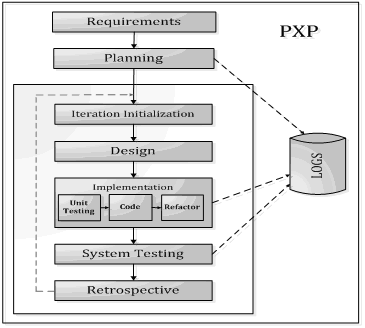
\includegraphics[width=0.5\textwidth]{imagenes/PXP-process-phases.png}
    \caption{Diagrama de las fases de metodología Personal Extreme Programming (PXP) }[22]
    \label{fig: diagrama}
\end{figure}

\subsubsection{Metodologías de evaluación}
 En esta sección se presentan las metodologías de evaluación a utilizar en el proyecto.

\subsubsubsection{Prueba de caja negra}
Las pruebas de caja negra se centran en evaluar el comportamiento funcional de la aplicación desde la perspectiva del usuario, sin considerar la estructura interna del código ni los algoritmos utilizados. Este enfoque permite validar que el sistema responde correctamente a los datos de entrada y cumple con los requisitos establecidos en la documentación técnica. Para ello, se diseñan casos de prueba basados en las especificaciones funcionales, verificando que las salidas obtenidas coincidan con las esperadas.[15]

\subsubsection{Prueba de usabilidad}
Las pruebas de usabilidad permiten validar la experiencia del usuario final con la aplicación desarrollada. Para este propósito, se aplicará la técnica System Usability Scale (SUS), una herramienta creada por John Brooke en 1986 y ampliamente utilizada en la industria del software. Esta prueba consiste en un cuestionario de 10 afirmaciones evaluadas mediante la Escala de Likert, donde los participantes expresan su nivel de acuerdo. A partir de estas respuestas, se calcula un puntaje total entre 0 y 100 que refleja la percepción de usabilidad: valores inferiores a 50 indican una experiencia inaceptable, entre 50 y 68 se consideran deficientes o mediocres, y puntuaciones superiores a 68 reflejan una aceptación adecuada del sistema por parte del usuario.[16]
\endgroup

\subsection{Diseño de software}

\subsubsection{Arquitectura fisíca}

\subsubsection{Arquitectura lógica}

\subsubsection{Modelo de datos}

\subsubsection{Mockups}

\subsection{Iteraciones}


\section{Bibliografia}
\begingroup
\small
\noindent [1] Fabricación y comercialización de muebles multifuncionales. \url{https://repositorio.uchile.cl/bitstream/handle/2250/146047/Vidal%20Castillo%20Rodrigo.pdf} \vspace{0.5em}

\noindent [2] Informes de Expertos, “Mercado de muebles en Chile 2024–2034: tendencias, oportunidades y pronóstico,” 2024. \url{https://www.informesdeexpertos.com/informes/mercado-de-muebles-en-chile} \vspace{0.5em}

\noindent [3] Cámara Nacional de Comercio, “Ventas presenciales del Comercio Minorista de la Región Metropolitana obtienen dispares resultados durante enero y febrero.” \url{https://cnc.cl/ventas-presenciales-del-comercio-minorista-de-la-region-metropolitana-obtienen-dispares-resultados-durante-enero-y-febrero} \vspace{0.5em}

\noindent [4] Cámara Nacional de Comercio, “Ventas presenciales minoristas de Valparaíso y La Araucanía positivas en 2025; Biobío con caídas.” \url{https://cnc.cl/los-dos-primeros-meses-del-2025-las-ventas-presenciales-minoristas-de-las-regiones-de-valparaiso-y-la-araucania-marcaron-resultados-positivos-mientras-que-biobio-registro-caidas} \vspace{0.5em}

\noindent [5] Autodesk, “AutoCAD.” \url{https://www.autodesk.com/latam/products/autocad/overview} \vspace{0.5em}

\noindent [6] IKEA, “IKEA Planner.” \url{https://www.ikea.com/cl/es/planners} \vspace{0.5em}

\noindent [7] Hexagon, “Cabinet Vision.” \url{https://hexagon.com/es/products/product-groups/computer-aided-manufacturing-cad-cam-software/cabinet-vision} \vspace{0.5em}

\noindent [8] Moblo App. \url{https://play.google.com/store/apps/details?id=fr.moblo&pli=1} \vspace{0.5em}

\noindent [9] Cut List Optimizer. \url{https://www.cutlistoptimizer.com} \vspace{0.5em}

\noindent [10] Trimble, “SketchUp for Web.” \url{https://sketchup.trimble.com/en/products/sketchup-for-web} \vspace{0.5em}

\noindent [11] OptiCutter. \url{https://www.opticutter.com} \vspace{0.5em}

\noindent [12] Asana, “¿Qué es Kanban?” \url{https://asana.com/es/resources/what-is-kanban} \vspace{0.5em}

\noindent [13] L. Williams, “Personal Extreme Programming: An Agile Process for Autonomous Developers,” ResearchGate. \url{https://www.researchgate.net/publication/229046039_Personal_Extreme_Programming-An_Agile_Process_for_Autonomous_Developers} \vspace{0.5em}

\noindent [14] Asana, “Lean Startup.” \url{https://asana.com/es/resources/lean-startup} \vspace{0.5em}

\noindent [15] Zaptest, “Pruebas de caja negra: tipos, procesos y herramientas.” \url{https://www.zaptest.com/es/pruebas-de-caja-negra-que-son-tipos-procesos-enfoques-herramientas-y-mucho-mas} \vspace{0.5em}

\noindent [16] QuestionPro, “Pruebas de usabilidad (SUS).” \url{https://www.questionpro.com/blog/es/pruebas-de-usabilidad/} \vspace{0.5em}

\noindent [17] Industria Manufacturera, “Procesos de fabricación de muebles: todo lo que necesitas saber.” \url{https://industriamanufacturera.com/procesos-de-fabricacion-de-muebles-todo-lo-que-necesitas-saber/} \vspace{0.5em}

\noindent [18] Subsecretaría de Telecomunicaciones de Chile, “Diagnóstico sobre las brechas de inclusión digital en Chile,” Subtel, Santiago, Chile, 2022. [Online]. Available: \url{https://www.subtel.gob.cl/plansocial/img/Diagnostico_inclusion_digital_vf.pdf} \vspace{0.5em}

\noindent [19] C. A. Rojas and M. E. González, “Adopción tecnológica en microempresas rurales: barreras y oportunidades,” Revista de Estudios Regionales, vol. 45, pp. 89–105, 2021. \vspace{0.5em}

\noindent [20] Cámara de Comercio de Santiago, “Informe sobre comportamiento del consumidor digital en Chile,” CCS, Santiago, Chile, 2022. [Online]. Available: \url{https://www.ccs.cl/informe-comportamiento-consumidor-digital-2022/} \vspace{0.5em}

\noindent [21] Industria Manufacturera, “Procesos de fabricación de muebles.” \url{https://industriamanufacturera.com/procesos-de-fabricacion-de-muebles-todo-lo-que-necesitas-saber/} \vspace{0.5em}

\noindent [22] Figura del proceso PXP. \url{https://www.researchgate.net/profile/Iva-Krasteva/publication/229046039/figure/fig1/AS:393822161915923@1470905928520/PXP-process-phases.png} \vspace{0.5em}

\endgroup
\end{document}
